\documentclass[10pt, handout]{beamer}
\usepackage{xmpincl}
\includexmp{license}
\usepackage[T1]{fontenc}
\usepackage[latin1]{inputenc}
\usepackage{ae}
\usepackage[french]{babel}
\usepackage{array, longtable}
\usepackage{tikz}
\usetikzlibrary{arrows,shapes,trees,fit,decorations.pathmorphing,backgrounds}
\usetheme{Antibes}
\setbeamertemplate{navigation symbols}{}

% for printing
\usepackage{pgfpages}
%\pgfpagesuselayout{2 on 1}[a4paper,border shrink=5mm]
%\pgfpagesuselayout{resize to}[a4paper,border shrink=5mm,landscape]


\usepackage{listings}
\usepackage{verbatim}
\makeatletter
\newwrite\lstvrb@out
\newenvironment{code}{%
  \begingroup
  \@bsphack
  \immediate\openout\lstvrb@out\jobname.lst
  \let\do\@makeother\dospecials\catcode`\^^M\active
  \def\verbatim@processline{%
    \immediate\write\lstvrb@out{\the\verbatim@line}}%
  \verbatim@start}{%
  \immediate\closeout\lstvrb@out
  \@esphack
  \endgroup

  \begin{alertblock}{}
    \lstinputlisting[language=java]{\jobname.lst}
  \end{alertblock}}
\makeatother

\lstset{language=java, basicstyle=\small, commentstyle=\color{blue}\textrm}

\title{Computer Science Introductory Course MSc - Software Engineering}

\subtitle{Lecture 6: GUI design with SWING}

\author[Pablo Oliveira]{Pablo Oliveira \texttt{<pablo@sifflez.org>}}
\institute{T\'el\'ecom ParisTech}

\date{}

\begin{document}
\begin{frame}
  \titlepage
\end{frame}

\begin{frame}
  \frametitle{Outline}
  \tableofcontents
\end{frame}

\section{JFrame}
\begin{frame}[fragile]
  \frametitle{Top-level container: JFrame}
  \begin{verbatim}
import javax.swing.*;
import java.awt.*;

class Test {
  public static void main(String[] args) {
    JFrame frame = new JFrame("This is a frame");
    frame.setDefaultCloseOperation(JFrame.EXIT_ON_CLOSE);
    frame.setPreferredSize(new Dimension(400, 200));
    frame.pack();
    frame.setVisible(true);
  }
}
\end{verbatim}
\begin{center}
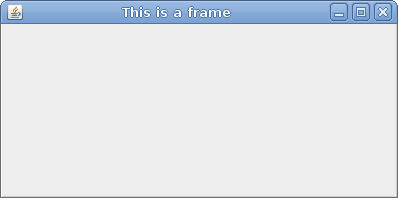
\includegraphics[width=0.6\linewidth]{frame}
\end{center}
\end{frame}

\section{Components}
\subsection{Adding components}
\begin{frame}[fragile]
  \frametitle{Adding components to our frame}
  \begin{verbatim}
public static void main(String[] args) {
  JFrame frame = new JFrame("This is a frame");
  frame.setPreferredSize(new Dimension(400, 200));
  frame.setDefaultCloseOperation(JFrame.EXIT_ON_CLOSE);

  JPanel panel = new JPanel();
  frame.setContentPane(panel);
  panel.add(new JLabel("Hello World!"));

  frame.pack();
  4frame.setVisible();
}
\end{verbatim}
\begin{center}
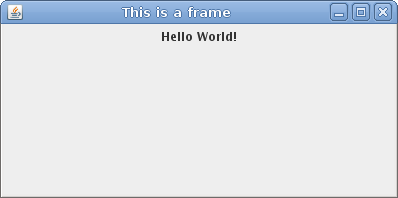
\includegraphics[width=0.6\linewidth]{label}
\end{center}
\end{frame}

\tikzstyle{level 1}=[level distance=3cm, sibling distance=1cm]
\tikzstyle{level 2}=[level distance=4cm, sibling distance=1.5cm]
\tikzstyle{level 3}=[level distance=3cm, sibling distance=1cm]

\subsection{Components Hierarchy}
\begin{frame}[fragile, shrink]
  \frametitle{Components Hierarchy}
\begin{center}
\begin{tikzpicture}[grow=right]
  \node {\verb!JComponent!}
  child {
    node {\verb!JTextComponent!}
    child{
      node {\verb!JTextArea!}
    }
    child{
      node {\verb!JEditorPane!}
      child{
        node{\verb!JTextPane!}
      }
    }
    child{
      node {\verb!JTextField!}
      child{
        node{\verb!JPasswordField!}
      }
    }
  }
  child{
    node {\verb!JComboBox!}
  }
  child{
    node {\verb!JLabel!}
  }
  child{
    node {\verb!JList!}
  }
  child{
    node {\verb!JMenuBar!}
  }
  child{
    node {\verb!JPanel!}
  }
  child{
    node {\verb!JPopupMenu!}
  }
  child{
    node {\verb!JScrollBar!}
  }
  child{
    node {\verb!JScrollPane!}
  }
  child {
    node {\verb!AbstractButton!}
    child {
      node {\verb!JToggleButton!}
      child{
        node {\verb!JCheckBox!}
      }
      child{
        node{\verb!JRadioButton!}
      }
    }
    child {
      node {\verb!JButton!}
    }
    child {
      node {\verb!JMenuItem!}
      child {
        node {\verb!JCheckBoxMenuItem!}
      }
      child {
        node {\verb!JMenu!}
      }
      child {
        node {\verb!JRadioButtonMenuItem!}
      }
    }
  };
\end{tikzpicture}
\end{center}
\end{frame}

\section{Layouts}
\begin{frame}[fragile]
  \frametitle{JPanel and layouts}
  \begin{itemize}
    \item \verb!JPanel! are containers that group and arrange other components.
    \item We add a component to a \verb!JPanel! with the \verb!.add(component)! method.
    \item Components inside a \verb!JPanel! are placed according to its
      \alert{layout}.
    \item Layouts implement the API interface \verb!LayoutManager!.
    \item We choose a JPanel's layout in its constructor \verb! new JPanel(new FlowLayout())!.
  \end{itemize}
\begin{center}
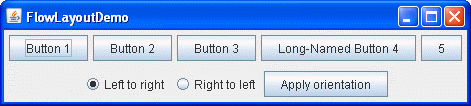
\includegraphics[width=0.6\linewidth]{FlowLayoutDemo1}
\end{center}
\end{frame}

\begin{frame}[fragile]
  \frametitle{Some examples of layouts}
  \begin{center}
    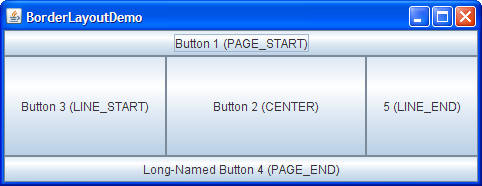
\includegraphics[width=0.6\linewidth]{BorderLayoutDemo}
  \end{center}
  \begin{center}
    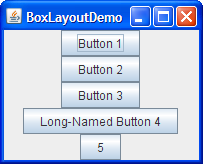
\includegraphics[width=0.4\linewidth]{BoxLayoutDemo}
  \end{center}
\end{frame}

\begin{frame}[fragile]
  \frametitle{More complex layouts}
  \begin{itemize}
    \item There are more complex layouts available, see:
      \verb!http://java.sun.com/docs/books/tutorial/uiswing/layout/!
    \item Using hierarchies of layouts, you can place your components very precisely.
  \end{itemize}
\end{frame}

\section{Event listeners}

\subsection{Clicking on a button}
\begin{frame}[fragile]
  \frametitle{Clicking on a button}
\begin{verbatim}
JButton button = new JButton("Hello!");
panel.add(button);
\end{verbatim}
\begin{center}
  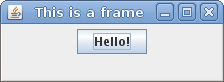
\includegraphics[width=0.38\linewidth]{beforeClick}
  
\includegraphics[width=0.4\linewidth]{afterClick}
\end{center}
\structure{How to react to an action from the user ?}
\end{frame}

\subsection{Listeners}
\begin{frame}[fragile]
  \frametitle{Listener interface}
\begin{verbatim}
import java.awt.event.*;
class ButtonListener implements ActionListener {
  JButton button;
  public ButtonListener(JButton button){
    this.button = button;
  }
  public void actionPerformed(ActionEvent e) {
    button.setLabel("Clicked");
  }
}

button.addActionListener(new ButtonListener(button));
\end{verbatim}
\end{frame}

\begin{frame}[fragile]
  \frametitle{Anonymous classes and listeners}
\begin{verbatim}
button.addActionListener(
  new ActionListener() {
    public void actionPerformed(ActionEvent e) {
      button.setLabel("Clicked");
    }
  });
\end{verbatim}
\end{frame}

\begin{frame}
  \frametitle{More on listeners}
  \begin{itemize}
    \item More details on listeners at:
      \verb!http://java.sun.com/docs/books/tutorial/uiswing/events/!
  \end{itemize}
\end{frame}

\section{Drawing}
\begin{frame}
  \frametitle{Drawing}
  \begin{itemize}
    \item Override the JComponent's method \verb!void paintComponent(Graphics g)!.
    \item This method is called each time the component must be redrawn.
    \item The \verb!Graphics! object lets you draw inside the Component.
    \item For a JFrame you can override the paint method.
    \item See example!
  \end{itemize}
\end{frame}

\section{Making your own components}
\begin{frame}
  \frametitle{Making your own components}
  \begin{itemize}
    \item As any other java class, \verb!JComponent! can be extended.
    \item This can be useful in many cases:
      \begin{itemize}
        \item Factorizing a component and its listeners in the same class.
        \item Changing the look of a component.
        \item Adding functionalities to a component.
      \end{itemize}
  \end{itemize}
\end{frame}
\begin{frame}[fragile, plain]
\begin{center}
  \tiny
  This work is licensed under a Creative Commons Attribution-Noncommercial-Share Alike 3.0 Unported License.
\vtop{
  \vskip-3ex
  \hbox{
    \includegraphics[height=0.4cm]{cc-logo}
  }
}
\end{center}
\end{frame}

\section{Exemple: Remember the Turtle ?}
\begin{frame}
  \frametitle{Exemple: Remember the Turtle ?}
  \begin{itemize}
  \item \alert{We are going to show, how the TurtleGraphics package was build.}
  \item Two classes \texttt{Sheet} and \texttt{Turtle}.
  \end{itemize}
\end{frame}

\begin{frame}[fragile]
  \frametitle{Sheet class : constructor 1/2}
  \begin{itemize}
    \item Create a JFrame and a Sheet.
    \item Put the Sheet inside the JFrame.
  \end{itemize}
\begin{verbatim}
/* A Sheet is a JComponent */
public class Sheet extends JComponent {
public Sheet(int width, int height) {
  /* Set the prefered size of the Sheet */
  this.setPreferredSize(new Dimension(width,height));

  /* Create a frame to show the sheet */
  JFrame f = new JFrame("Turtle");
  f.setDefaultCloseOperation(JFrame.EXIT_ON_CLOSE);

  /* Put the sheet inside the JFrame */
  f.setContentPane(this);
  f.pack();
  f.setVisible(true);
  ...
\end{verbatim}
\end{frame}

\begin{frame}[fragile]
  \frametitle{Sheet class : constructor 2/2}
  \begin{itemize}
    \item Create a list to keep turtles.
    \item Create an image for the turtles to draw in.
  \end{itemize}
\begin{verbatim}
  /* Create a list to keep the turtles */
  turtles = new LinkedList<Turtle>();

  /* Create an image for the turtles to draw in */
  offscreen = new BufferedImage(width,height,
                                BufferedImage.TYPE_INT_RGB);

  /* Set the turtle coordinate system */
  gra = (Graphics2D) offscreen.getGraphics();
  gra.translate(width/2,height/2);
  gra.scale(1,-1);
\end{verbatim}
\end{frame}

\begin{frame}
  \frametitle{Could we draw directly on the Sheet ?}
  \begin{itemize}
    \item Every JComponent, can be drawn onto with the method
      \texttt{paint(Graphics g)}: So why are we not drawing directly
      on the sheet ?
    \item Problems:
      \begin{itemize}
      \item \alert{Drawing in a JComponent directly may cause flickering,
          double buffering.}
      \item \alert{When moving the Sheet around, resizing it, the drawings
        goes away. Using the \texttt{offscreen} image buffer allows us to
        implement persistant graphics.}
      \end{itemize}
  \end{itemize}
\end{frame}

\begin{frame}[fragile,shrink]
  \frametitle{So how Turtles draw on the offscreen buffer ?}
\begin{verbatim}
public class Sheet {
  protected void drawLine(double ax, double ay,
                          double bx, double by,
                          Color color) {
    gra.setColor(color);
    gra.draw(new Line2D.Double(ax,ay,bx,by));
  }
}

public class Turtle {
  public void advance(double steps) {
    double newx = x + steps*Math.cos(theta);
    double newy = y + steps*Math.sin(theta);
    if (pen_down && sheet != null) {
      sheet.drawLine(x,y,newx,newy, penColor);
    }
    x = newx;
    y = newy;
    sheet.repaint();
  }
}
\end{verbatim}
\end{frame}

\begin{frame}[fragile, shrink]
  \frametitle{Finally: Blitting the offscreen image and drawing the Turtles}
\begin{verbatim}
public class Sheet {
public void paint(Graphics g) {
  Graphics2D g2 = (Graphics2D) g;

  /* draw the sheet image */
  g2.drawImage(offscreen,0,0,this);

  /* set turtle coordinate system */
  g2.translate(width/2,height/2);
  g2.scale(1,-1);

  /* draw each turtle */
  Iterator<Turtle> it = turtles.iterator();
  while(it.hasNext()) {
    Turtle t = it.next();
    t.drawTurtle(g2);
  }
}
}
\end{verbatim}
\end{frame}

\begin{frame}[fragile]
  \frametitle{How does a Turtle draws itself ?}
\begin{verbatim}
public class Turtle {
  ...
  turtleColor = Color.BLUE;
  turtleShape = new Polygon(new int[] {0,0,10},
                            new int[] {3,-3,0}, 3);
  ...
  protected void drawTurtle(Graphics2D graphics) {
    graphics.setColor(turtleColor);
    graphics.translate(x,y);
    graphics.rotate(theta);
    graphics.fill(turtleShape);
  }
}
\end{verbatim}
\end{frame}

\end{document}
